\section{Introduction}\label{sec:introduction}


The first application of the Cahn-Hilliard (CH) problem appeared when modelling phase separation of two-component incompressible fluids \cite{cahn1958free, cahn1959free, cahn1961spinodal}, but was quickly generalized to handle multi-component system
as well \cite{bosch2015fractional, eyre1993systems, toth2016phase, miranville2017cahn}. In engineering, CH is the critical component in
the phase-field model, a mathematical framework to model transitions and interface dynamics in materials and fluid dynamics \cite{steinbach2009phase, chen2002phase}.
From this, the equation found many interesting applications for a wide variety of problems. To mention a few, we have
multiphase fluid dynamical problems \cite{badalassi2003computation, li2016lattice, kim2012phase, shen2010phase}, solidification of binary or multi-component alloys \cite{kim1999phase, echebarria2004quantitative}, and continuum modelling of fracture dynamics in
materials \cite{kuhn2010continuum, li2015phase}. Perhaps an unexpected application is that CH can be used for in painting when recovering damaged parts of an image \cite{bertozzi2006inpainting, burger2009cahn, bosch2015fractional, brkic2020image}
and modelling the origin of the irregular structure in Saturn's rings \cite{tremaine2003origin}.
CH is also essential in many areas of biology and medicine. For example, from a macroscopic viewpoint, CH is a great tool to model tumour growth, wound healing and brain tumours \cite{agosti2017cahn, cristini2009nonlinear}.
On the microscopic level on the biomembrane, there is an ongoing debate about the existence of the accumulation of lipids into so-called lipid rafts, which serve as a rigid platform for proteins with
special properties such as signalling and intercellular trafficking \cite{ levental2020lipid, hancock2006lipid, munro2003lipid, simons1997functional}. It turns out that the hypothesis can be tested by modelling the problem as a separation problem using
CH \cite{miller2020divide, garcke2016coupled, yushutin2019computational}.

\subsection{The Cahn Hilliard Problem}%
\label{sub:the_equations}

The CH problem comes in many variants depending on its application, but we will in this report on the binary mixture version \cite{miranville2017cahn}. Let $\Omega \subset  \mathbb{R} ^{d} $ be a compact set for $d=2,3$ with a sufficiently smooth boundary
$\Gamma $,  see Figure \ref{fig:domain_construction}. We define the time duration parameter $T \in  [0,\infty) $ and the
so-called unknown phase-field function as the
mapping $u: \left[ 0, T \right] \times \Omega  \to \left[ -1,1 \right]  $, which is denoted as the local difference of a binary mixture of two concentrations $c_{A}, c_{B} \in \left[ 0,1\right] $ s.t. $u = c_{A} -c_{B}$ and $c_{A} + c_{B} = 1$. Remark that if a local point exists so $u$ has the extreme value $-1$, then it implies that the particular point has $100\%$ concentration $c_{A}$ and vice-versa for $c_{B}$. On the other hand, if $u$ is zero, it implies that the mixture is $50\% - 50\%$.

\begin{figure}[htpb!]
    \centering
    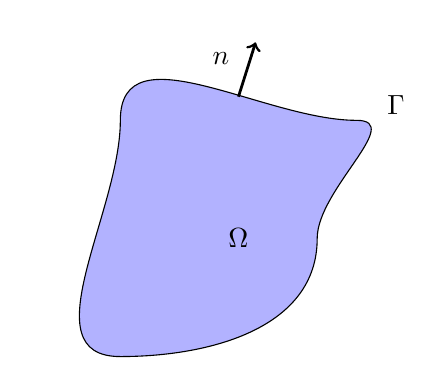
\begin{tikzpicture}
        % Define points for square
        \coordinate (A) at (-1.5,-1.5);
        \coordinate (B) at (1.0,0.0);
        \coordinate (C) at (1.5,1.5);
        \coordinate (D) at (-1.5,1.5);

        \filldraw[fill=blue!30,draw=black] (A) to[out=0,in=-90] (B) to[out=90,in=0] (C) to[out=180,in=90] (D) to[out=-90,in=180] cycle;
\draw[->, line width=1.0pt] ({1.8*cos(90)}, { 1.8*sin(90) }) -- ({ 2.5*cos(85)  }, { 2.5*sin(85)  }) node[below left, xshift=-0.2cm] {$n $};

        \node at (0,0) {$\Omega$};
        \node at (2,1.7) {$\Gamma$};

    \end{tikzpicture}
    \caption{Illustration of the physical domain $\Omega$ for $d=2$ , the boundary $\Gamma$ and the corresponding normal vector $n$.}
    \label{fig:domain_construction}
\end{figure}

For an isotropic
binary mixture non-uniform, the standard Ginzburg-Landay free energy functional is given by \[
E( u)  = \int_{\Omega }^{} \frac{\varepsilon ^2}{2} \abs{ \nabla u } ^2 + F( u) dx
\]
The nonlinear function $F( u) $ is denoted as the (Helmholtz) free energy density associated with the interaction dynamics between the components and thus comes in many forms depending on the thermodynamic properties, see \cite{miranville2017cahn}.
However, we will in this article assume that $F( u) = ( 1 / 4 ) ( 1- u^2) ^{4} $.
We choose to define the chemical potential $\mu $ as the variational derivative,
\[
\mu = \frac{ \delta E( u) }{ \delta  u} = f( u)  - \varepsilon ^{2} \Delta c .
\]
where we used the notation $f( u) = F'( u) $.
First of all, to require local mass conservation, we may enforce the continuity equation, that is \[
\partial _{t} u + \nabla \cdot \mathcal{J}  = 0,
\]
where $J$ denotes the flux governed by the physical dynamics. Hence, this naturally leads to the no-flux and the Neumann boundary conditions,
\begin{equation}
\label{eq:conservation}
    \begin{split}
\mathcal{J}  \cdot n & = 0 \text{ on } \Gamma \\
\partial _{n} u & = 0 \text{ on } \Gamma
    \end{split}
\end{equation}
 A well-accepted law for the flux is that it is proportional to the chemical energy gradient, $\mathcal{J} = - M  \nabla \mu  $ for a parameter $M$.
Thus, we finally have the strong form Cahn-Hilliard equation. Let $ u( x,0) =  u_{0}$ then is the dynamics on the form,

\begin{equation}
\label{eq:strongch}
    \begin{split}
\partial _{t} u  = \Delta ( f( u)  - \varepsilon ^2 \Delta u ) &\quad \text{ in } \Omega  \\
\partial _{n} u = 0 \quad &\text{ on } \Gamma  \\
\partial _{n}(f( u)  - \varepsilon ^2 \Delta u )  = 0 \quad &\text{ on } \Gamma  \\
    \end{split}
\end{equation}

Based on these laws and the boundary conditions, it becomes evident that the energy functional serves as a Lyapunov function in the sense that its time derivative is monotonically decreasing and that the global mass concentration is zero, i.e.
\[
    \begin{split}
\frac{d}{dt} E( u)  \le  0 \text{ and }\frac{d}{dt} \int_{\Omega }^{}  u dx = 0.
    \end{split}
\]
Remark that the inequality computation utilizes the assumption of $M$ to be constant, and both equations require the no-flux boundary condition, $\mathcal{J} \cdot n = 0$.
For details, see \cite[Equation 17 ]{lee2014physical} and \cite[Equation 1.7]{garcke2020weak}.
This is useful since we expect $E( u( \cdot , t_{2}) ) \le  E( u( \cdot , t_{1}) ) $ for $0 < t_{1} < t_{2} $ and that the global mass is conserved, \[
\int_{\Omega }^{} u ( x,t)  dx = \int_{\Omega }^{} u_{0}(x)  dx.
\]
The properties under consideration serve as a theoretical foundation for establishing the existence, uniqueness, and long-term behaviour of the CH problem. Consequently, these properties are well-comprehended from a mathematical standpoint. For
references, see \cite{abels2007convergence, cherfils2011cahn, elliott1986cahn}.

\subsection{Numerical Methods}%
\label{sub:numerical_methods}

One of the key challenges with the CH problem is that it involves fourth-order spatial derivatives. It has, for simple domains, successfully been implemented using Finite Difference Methods \cite{furihata2001stable,
cheng2019energy} and Spectral Methods \cite{liu2003phase, he2009class}. However, these methods are generally constrained to simple domains (with some notable exceptions \cite{li2013conservative, shen2009efficient, feng2009fourier}).

As a further evolution to address the CH problem, it is common to consider a corresponding biharmonic (BH) problem as a numerical testbed in the spatial direction. This problem is defined as follows,
\begin{equation}
\label{eq:BH-problem}
\begin{split}
    \alpha u + \Delta ^2 u  & = f( x) \quad \text{in }  \Omega, \\
    \partial _{n} u & = g_{1}( x)  \quad \text{on } \Gamma,   \\
    \partial _{n} \Delta  u & = g_{2}( x)  \quad \text{on } \Gamma.   \\
\end{split}
\end{equation}
Here is the functions a mapping $f,g_{1} ,g_{2}: \Omega  \to \mathbb{R} $ and the constant $\alpha  $ is a real number s.t. $\alpha >0$.
The BH problem holds relevance since it is provide a proper spatial-integration test framework prior to moving on solving the non-linearities and time-integration.

The early Finite Element Methods (FEM) for CH were proposed in \cite{elliott1987numerical, elliott1986cahn} utilizing global $C^{1}$ and $C^{2}$ in one spatial dimension, but later it has been shown that making $C^{1}$ (or higher order) elements are far from trivial. For
reference, see \cite{kapl2021family, percell1976cubic, argyris1968tuba}.

% Describe the isogeometric analysis and virtual elements methods as alternatives.
There exist several promising alternative methods that guarantee $C^{1}$ continuity, and these have shown potential for solving the CH problem. A notable mention is isogeometric analysis (IGA), a technique that leverages Non-Uniform
Rational B-Splines (NURBS) to efficiently handle complex geometries and smooth boundaries without the need for mesh refinement. Thus, IGA makes a desirable alternative for problems dealing with intricate and smooth domains
\cite{hughes2005isogeometric}. Specifically for the CH problem, has IGA successfully been implemented \cite{kastner2016isogeometric, gomez2008isogeometric}. Recent results have shown that investigations on unfitted versions of IGA
\cite{zhao2017variational} and its applicability to moving surfaces \cite{zimmermann2019isogeometric} also is possible.
Another rising method is the virtual finite element method (VFEM), which has applied so-called virtual $C^{1}$ elements to handle the continuity requirement \cite{antonietti2016c}.

\begin{figure}[h!]
    \centering
    % First TikZ picture
    \begin{minipage}{0.45\textwidth}
        \centering
        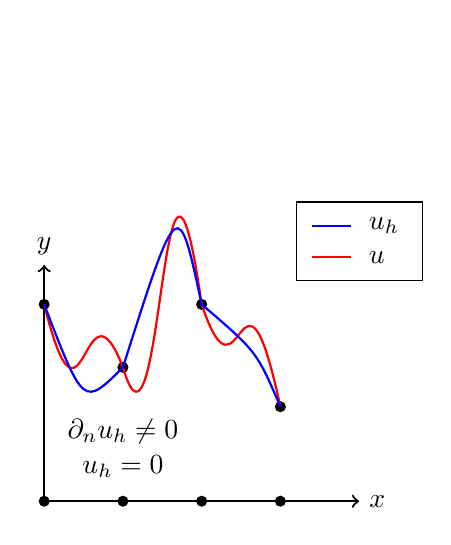
\begin{tikzpicture}
            % Draw x-axis
            \draw[->, thick] (0,0) -- (4,0) node[right] {$x$};
            % Draw y-axis
            \draw[->, thick] (0,0) -- (0,3) node[above] {$y$};

            % Draw nodes at center, A, B, and C with arbitrary y-values
            \foreach \x/\y in {0/2.5, 1/1.7, 2/2.5, 3/1.2} {
                \fill (\x,\y) circle (2pt); % Filled nodes with y-values
                \fill (\x,0) circle (2pt); % Filled circles on x-axis
            }

            % Exact solution
            \draw[red, thick] (0,2.5) .. controls (0.5,0.5) and (0.5,3) .. (1,1.7) .. controls (1.5,0) and (1.5,6) .. (2,2.5) .. controls (2.5,1) and (2.5,3.5) .. (3,1.2);
            \node at (1,0.6) [above] {$\jump{ \partial _{n} u_{h} } \neq 0$};
            \node at (1,0.7) [below] {$\jump{ u_{h} }   = 0$};

            %% Second
            \draw[blue, thick] (0,2.5) .. controls (0.5,1.2) .. (1,1.7)
            .. controls (1.7,3.9) .. (2,2.5)
            .. controls (2.7,1.9) .. (3,1.2); Second

            \draw (3.2,2.8) rectangle (4.8,3.8); % Legend box
            \draw[blue, thick] (3.4,3.5) -- (3.9,3.5); % Blue line for u_h
            \draw[red, thick] (3.4,3.1) -- (3.9,3.1); % Red line for u
            \node[anchor=west] at (4.0,3.5) {$u_h$}; % Label for u_h
            \node[anchor=west] at (4.0,3.1) {$u$}; % Label for u

        \end{tikzpicture}
    \end{minipage}
    \hfill
    % Second TikZ picture
    \begin{minipage}{0.45\textwidth}
        \centering
    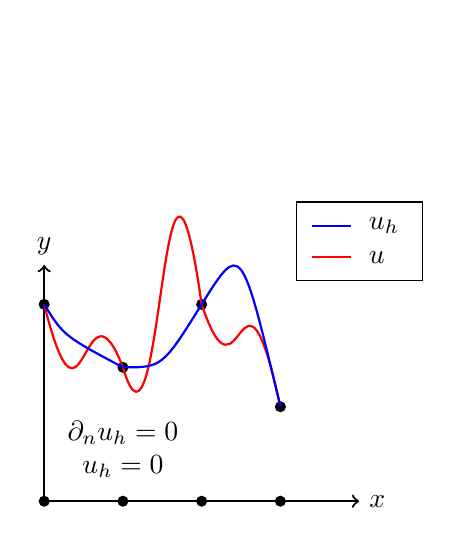
\begin{tikzpicture}
        % Draw x-axis
        \draw[->, thick] (0,0) -- (4,0) node[right] {$x$};
        % Draw y-axis
        \draw[->, thick] (0,0) -- (0,3) node[above] {$y$};

        % Draw nodes at center, A, B, and C with arbitrary y-values
        \foreach \x/\y in {0/2.5, 1/1.7, 2/2.5, 3/1.2} {
            \fill (\x,\y) circle (2pt); % Filled nodes with y-values
            \fill (\x,0) circle (2pt); % Filled circles on x-axis
        }

        % Exact solution
        \draw[red, thick] (0,2.5) .. controls (0.5,0.5) and (0.5,3) .. (1,1.7) .. controls (1.5,0) and (1.5,6) .. (2,2.5) .. controls (2.5,1) and (2.5,3.5) .. (3,1.2);
        \node at (1,0.6) [above] {$\jump{ \partial _{n} u_{h} } = 0$};
        \node at (1,0.7) [below] {$\jump{ u_{h} }   = 0$};

        % Second
        \draw[blue, thick]
        (0,2.5) .. controls (0.25,2.1) .. (1,1.7)
        (1,1.7) .. controls (1.5,1.7) .. (2,2.5)
        (2,2.5) .. controls (2.5,3.3) .. (3,1.2);

        \draw (3.2,2.8) rectangle (4.8,3.8); % Legend box
        \draw[blue, thick] (3.4,3.5) -- (3.9,3.5); % Blue line for u_h
        \draw[red, thick] (3.4,3.1) -- (3.9,3.1); % Red line for u
        \node[anchor=west] at (4.0,3.5) {$u_h$}; % Label for u_h
        \node[anchor=west] at (4.0,3.1) {$u$}; % Label for u
    \end{tikzpicture}
    \end{minipage}
\caption{ Illustration of global $C^{0}$ continuous elements (left) and global $C^{1}$ elements (right) in 1 dimension. Here is $u$ the exact solution and $u_{h}$ the approximated solution. We define the jump between the elements as $ \jump{ u_{h} } = u_{+} - u_{-}$.}
\label{fig:global_C0}
\end{figure}

An alternative approach is to avoid global $C^1$ continuity weakend it to global $C^{0}$ continuity, see Figure \ref{fig:global_C0} . As a result, this strategy has led to the development of two distinct families of methods for solving the CH problem.
% Paragraph of CIP
The first involves the Continuous Interior Penalty (CIP) methods, which uses the standard weak formulation but penalizes the discontinuity of the derivative between elements as a form of regularization. The method has been designed for several interesting
stable variants for the BH problem, that is \cite{brenner2012, brenner2012quadratic, brenner2012quadratic_kirk, mu2014weak, georgoulis2009discontinuous}.
This method is advantageous due to its symmetry and relationship with discontinuous Galerkin (DG) methods \cite{di2011mathematical}, renowned for their natural way of handling inhomogeneous boundary conditions, flexibility with unstructured meshes, efficient parallelization, and strong stability. This connection lends robust stability analysis tools, making the method highly suitable for intricate computational problems.
The CIP formulation has also then been adapted to solve CH by applying the Newton-Raphson scheme to handle the non-linearities \cite{wells2006discontinuous} or utilizing an implicit-explicit (IMEX) time integration scheme, where the stiff part is treated implicitly (such as backward Euler) and the nonlinear part explicitly (such as the forward
Euler or explicit Runge-Kutta) \cite{ feng2007fully}.

Another popular variant is to rewrite the BH problem as a system of second-order problems in a mixed formulation. This strategy not only broadens the problem's flexibility but also provides a more natural means to incorporate boundary conditions,
see \cite{falk1978approximation,
ciarlet1974mixed, gudi2008mixed, cheng2000some}. This approach also leverages the general saddle point theory for mixed
FEM methods, which provide a mathematical framework to ensure numerical stability \cite{john2016finite}.
Moreover, this approach adapts well to the CH problem \cite{wells2006discontinuous,feng2004error}, and some methods even apply a so-called convex splitting scheme approach in a way that preserves the convexity of the energy functional, making the
system easier to solve \cite{diegel2015analysis, brenner2018robust}.
A combination of these methods, the DG and mixed formulation for the CH problem, has recently been considered \cite{chave2016hybrid, medina2022stabilized}.

\begin{figure}[h!]
    \centering
    % First TikZ picture
    \begin{minipage}{0.45\textwidth}
        \centering
        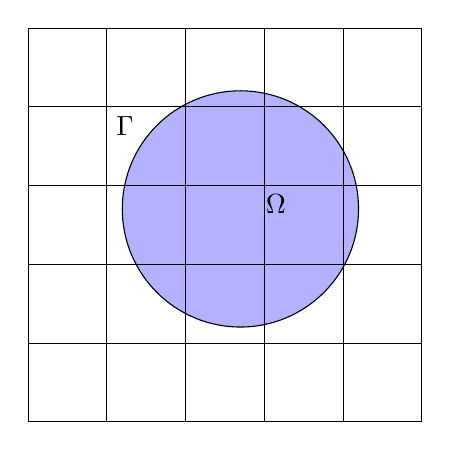
\begin{tikzpicture}
            \draw[fill=blue!30] (0.2, 0.2) circle (1.5cm);
            % Background mesh
            \foreach \i in {-2.5, -1.5, ..., 2.5} {
                \draw[line width=0.1pt, shift={(-2.5,\i)}] (0,0) -- (5,0);
                \draw[line width=0.1pt, shift={(\i,-2.5)}] (0,0) -- (0,5);
            }
            % Labels
            \node[below right] at (0.4,0.5) {$\Omega $};
            \node[below right] at (-1.5,1.5) {$\Gamma $};
            % \draw[blue, thick] (-2.5, -2.5) rectangle (2.5, 2.5);
        \end{tikzpicture}
    \end{minipage}
    \hfill
    % Second TikZ picture
    \begin{minipage}{0.45\textwidth}
        \centering
        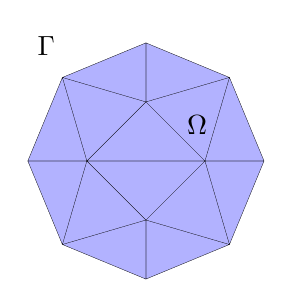
\begin{tikzpicture}
            % FIGURE OF FITTED MESH
            % Boundary points
            \foreach \i in {0, 45, ..., 315} {
                \coordinate (boundary-\i) at (\i:1.5cm);
            }
            % Interior points
            \coordinate (interior-1) at (0.75, 0);
            \coordinate (interior-2) at (-0.75, 0);
            \coordinate (interior-3) at (0, 0.75);
            \coordinate (interior-4) at (0, -0.75);

            % Create a cycle connecting all the boundary points
            \fill[blue!30] (boundary-0) -- (boundary-45) -- (boundary-90) -- (boundary-135) -- (boundary-180) -- (boundary-225) -- (boundary-270) -- (boundary-315) -- cycle;

            % Labels
            \node[below right] at (0.4,0.7) {$\Omega $};
            \node[below right] at (-1.5,1.7) {$\Gamma $};

            % Triangulation (manually specified)
            \draw[line width=0.1pt] (boundary-0) -- (boundary-45) -- (interior-1) -- cycle;
            \draw[line width=0.1pt] (boundary-45) -- (boundary-90) -- (interior-3) -- cycle;
            \draw[line width=0.1pt] (boundary-90) -- (boundary-135) -- (interior-3) -- cycle;
            \draw[line width=0.1pt] (boundary-135) -- (boundary-180) -- (interior-2) -- cycle;
            \draw[line width=0.1pt] (boundary-180) -- (boundary-225) -- (interior-2) -- cycle;
            \draw[line width=0.1pt] (boundary-225) -- (boundary-270) -- (interior-4) -- cycle;
            \draw[line width=0.1pt] (boundary-270) -- (boundary-315) -- (interior-4) -- cycle;
            \draw[line width=0.1pt] (boundary-315) -- (boundary-0) -- (interior-1) -- cycle;

            % Triangulation between interior points
            \draw[line width=0.1pt] (interior-1) -- (interior-2) -- (interior-3) -- cycle;
            \draw[line width=0.1pt] (interior-1) -- (interior-2) -- (interior-4) -- cycle;

            % \draw[blue, thick] (-2.5, -2.5) rectangle (2.5, 2.5);

        \end{tikzpicture}
    \end{minipage}
\caption{Mesh comparison: unfitted mesh (left) adheres to domain and boundary, while fitted mesh (right) employs a triangular mesh for polygonal approximation of the circular domain.}
\label{fig:domain_mesh}
\end{figure}

Creating a high-quality mesh in 2- and 3-dimensional for realistic problems is a challenging task that can take a reasonable time in the simulation workflow and is hard to scale properly on distributed platforms and thus not that suitable for moving
domains, very complex meshes or smooth boundaries. An interesting class to approach the problem is the so-called unfitted finite element method, which utilizes a background mesh and does not align with the physical boundary. For an illustration
see Figure \ref{fig:domain_mesh}.
This greatly reduces the need to generate an unstructured mesh and makes it very applicable for parallelization and moving domains
since it avoids the need of remeshing entirely. However, without paying attention to the so-called cut cells, which are the elements intersecting with the boundary, the method quickly leads to instability and ill-conditioning.
One of the methods to counter this is the cut finite element method (CutFEM), where the focus is to penalize the cut-cells weakly by adding an additional ghost penalty term to ensure stability and well-posedness \cite{burman2015cutfem}. Notably, there exist related methods, sometimes considered equivalent, named Extended FEM and Trace FEM \cite{cai2021nitsche,zonca2018unfitted}.
This has been successfully implemented for the BH problem for the
mixed formulation \cite{cai2023nitsche} and the CIP formulation \cite{chen2023arbitrary, cai2021nitsche}. However,  both implementations are considering an interface problem between two domains. Specifically for the CH problem, the mixed formulation \cite{karatzas2021reduced} has been shown to be successful.
 Aggregated unfitted finite element method (AgFEM) is a close relative to CutFEM and has also shown to
be promising \cite{badia2018aggregated, badia2022linking}. The method is an alternative way to the ghost penalty, which instead applies a so-called cell aggregation with respect to a cut cell ( assuming each cell has enough support with interior elements) and,
thus, the badly cut cells are removed, ensuring robustness and well-posedness.




\subsection{Outline of the report}%
\label{sub:outline_of_the_report}

This report is a novel stabilized cut continuous interior penalty method (CutCIP) that utilizes the CutFEM framework to handle complex domains and the CIP formulation for its elegant formulation to handle fourth-order spatial derivatives, to solve
the CH problem. We will name the cut continuous interior penalty method (CutCIP) method. In the first section prove that the method is stable and has optimal
convergence for the BH problem, and then extend the method to handle the CH problem. We will then provide numerical examples.
